% Pandoc template for docs/conclusions.tex (LuaLaTeX + biblatex/biber). Used by docs/build.sh.
\documentclass[11pt,a4paper]{article}
\usepackage[margin=2.6cm]{geometry}
\usepackage{fontspec}
\setmainfont{Libertinus Serif}
\setsansfont{Libertinus Sans}
\setmonofont{Libertinus Mono}[Scale=MatchLowercase]
\usepackage[british]{babel}
\usepackage{csquotes}
\usepackage{microtype}
\usepackage{xcolor}
\definecolor{link}{HTML}{0072B2}
\usepackage{graphicx}
\usepackage{longtable,booktabs,array,calc,etoolbox}
\makeatletter
\patchcmd\longtable{\par}{\if@noskipsec\mbox{}\fi\par}{}{}
\newsavebox\pandoc@box
\newcommand*\pandocbounded[1]{%
  \sbox\pandoc@box{#1}%
  \Gscale@div\@tempa{\textheight}{\dimexpr\ht\pandoc@box+\dp\pandoc@box\relax}%
  \Gscale@div\@tempb{\linewidth}{\wd\pandoc@box}%
  \ifdim\@tempb\p@<\@tempa\p@\let\@tempa\@tempb\fi
  \ifdim\@tempa\p@<\p@\scalebox{\@tempa}{\usebox\pandoc@box}\else\usebox{\pandoc@box}\fi}
\def\fps@figure{htbp}
\makeatother
\providecommand{\tightlist}{\setlength{\itemsep}{0pt}\setlength{\parskip}{0pt}}
\usepackage[font=small,labelfont=bf,labelsep=period]{caption}
\setlength{\parskip}{0.4em}
\setlength{\parindent}{0pt}
\setlength{\emergencystretch}{3em}
\usepackage[backend=biber,style=authoryear-comp,maxcitenames=2,uniquename=false,uniquelist=false,dashed=false]{biblatex}
\addbibresource{refs.bib}
\usepackage[hidelinks]{hyperref}
\hypersetup{colorlinks=true,linkcolor=link,citecolor=link,urlcolor=link,
  pdftitle={Did we listen to Joelle Pineau in 2018?},pdfauthor={Warith
Harchaoui},pdflang={en-GB}}
\IfFileExists{xurl.sty}{\usepackage{xurl}}{}

\title{\textbf{Did we listen to Joelle Pineau in 2018?}\\[0.4em]\large A
survey revisited. Every flaw she exposed in 2018, measured in the papers
of 2018 to 2026 and in our own experiments}
\author{Warith Harchaoui}
\date{9 November 2026, interim state}

\begin{document}
\maketitle

\section*{Summary}\label{summary}
\addcontentsline{toc}{section}{Summary}

In 2018, the researcher Joelle Pineau gave two talks at the largest
conferences in artificial intelligence. With numbers in hand, she showed
why the results of a field then at the height of its glory were hard to
believe. That field was deep reinforcement learning, which teaches a
machine to act by trial and error. She listed sixteen flaws. Papers came
without their code. Settings stayed secret. Competing methods were tuned
less carefully than the method being defended. Experiments rested on too
few runs, of which the best were kept. Comparisons went without a
statistical test. Agents were even evaluated in the very situations used
to train them
\autocite{pineau2018iclr,pineau2018neurips,henderson2018matters}.

This document goes through the whole list, flaw by flaw. Each time it
asks the same question: eight years on, did we listen to her? Two
instruments answer. The first is a survey: we reread 50 randomly drawn
papers from 2025 and 2026 with Pineau's reading grid, plus 12 papers
from 2018 to check that our reading recovers her figures. The second
gathers experiments: we rerun those of 2018 with the algorithms of 2026,
writing the protocol before the first training run.

Of sixteen flaws, only one was clearly heeded: 70\% of papers now
evaluate their agents on held-out situations, against 10\% in 2018. One
went backwards: the settings of competing methods now appear in only
18\% of papers, against 60\% in 2018. Three have not moved: the
statistical test (4\% of papers), the description of how a method gets
tuned (27\%) and the number of runs, which half of the papers leave
unstated. Our experiments qualify the most famous flaw. Two groups of
five runs of the same program, drawn at random, fool a statistical test
in only 1.2\% of cases. The test gets fooled when the runs are sorted
(31\%) or when the best ones are kept (+33\%). The experiments also
confirm the least visible flaw: the badly tuned baseline in our own
experiment was us. Six flaws remain to be measured: this document says
how.

\section{Two talks in 2018}\label{two-talks-in-2018}

\textbf{Vancouver, then Montreal.} In spring 2018, Joelle Pineau, a
professor at McGill University in Montreal and head of Facebook's
artificial intelligence research lab in that city, takes the stage at
ICLR (\emph{International Conference on Learning Representations}) in
Vancouver. In December she gives an expanded version of the talk at
NeurIPS (\emph{Neural Information Processing Systems}) in Montreal.
ICLR, NeurIPS and ICML (\emph{International Conference on Machine
Learning}) are the three leading conferences where machine learning
research gets published. Her talk is titled ``Reproducibility,
Reusability, and Robustness in Deep Reinforcement Learning''.

\textbf{A simple question.} When one team publishes a result, does
another team that follows the recipe get the same one? Pineau starts
from a survey by the journal \emph{Nature}: of 1,576 researchers across
all disciplines, more than 70\% said they had already failed to
reproduce a colleague's experiment \autocite{baker2016reproducibility}.
She then quotes a sentence written in 1995 by two Stanford
statisticians, Buckheit and Donoho: a scientific article about
computation is only the advertising for the research, the research
itself being the code and the data that produce the figures
\autocite{buckheit1995wavelab}. Then, figure after figure, she shows
what her own field lacks to deserve trust. Most of the figures come from
a paper by her team, signed by Peter Henderson and co-authors
\autocite{henderson2018matters}.

\textbf{What we make of these talks.} Eight years have passed. The field
has changed in size and in terrain. The conferences have adopted the
checklist Pineau proposed \autocite{pineau2021improving}. We want to
know what it changed in the papers themselves. So we take her list of
flaws as a grid and apply it to today's papers, then to our own
experiments. That was the rule she asked for: criticism applies to
oneself first.

\section{What you need to know to follow
along}\label{what-you-need-to-know-to-follow-along}

This document is written for readers who have never trained an agent.
Six notions cover everything that follows.

\textbf{Reinforcement learning.} A program, the agent, acts in a world,
the environment. At each step the agent observes a situation, chooses an
action and receives a numerical reward. It looks for the way of acting,
called a policy, that brings in the most reward overall. Our running
example is called HalfCheetah: an articulated cheetah drawn in two
dimensions inside a physics simulator. The agent drives the cheetah's
six joints and earns a reward whenever the cheetah moves forward. At
first the cheetah twitches. After a million steps it runs. We speak of
deep reinforcement learning (abbreviated RL from here on) when the
policy is a neural network.

\textbf{The random seed.} Training draws many numbers at random: the
network's starting weights, the exploratory actions, the cheetah's
starting position. A computer builds this randomness from a starting
number, the random seed. Same program, same random seed: same result.
Same program, another random seed: another result. In this document, a
``run'' means one complete training with a given random seed.

\textbf{The hyperparameter.} The network learns its weights unaided.
Other settings stay in the experimenter's hands: the learning rate, the
size of the network, the number of examples processed together. These
are the hyperparameters. The result depends heavily on them.

\textbf{The baseline.} To show that a new method does better, a paper
compares it with existing methods, called baselines. The comparison is
fair when every method has received the same care in tuning.

\textbf{The benchmark.} A benchmark is a set of standard tasks on which
everyone compares results. For the RL of 2018, the cheetahs, hoppers and
walkers of the MuJoCo simulator (\emph{Multi-Joint dynamics with
Contact}) \autocite{todorov2012mujoco} served as the benchmark. For the
language models of 2026, benchmarks are collections of mathematics
problems with their solutions.

\textbf{The statistical test and the confidence interval.} Two averages
always differ a little. A statistical test puts a number on the
probability of observing a gap at least that large if the two methods
were in fact equivalent: this number is the p-value. By convention, p
\textless{} 0.05 gets the gap declared ``significant''. A 95\%
confidence interval gives a range of values compatible with the data:
the wider it is, the less certain the measurement. We use the Wilson
interval, suited to proportions computed on few papers
\autocite{wilson1927probable}.

\section{The sixteen flaws of 2018}\label{the-sixteen-flaws-of-2018}

Pineau backs every flaw with an example, often with a figure. We
recorded the flaws in the order of her two talks, then sorted them into
four families. For each one, this document says what it is, why it
distorts a result and what Pineau showed about it. The labels F1 to F16
serve only to find a flaw in the tables.

\subsection{The materials: what rerunning an experiment
takes}\label{the-materials-what-rerunning-an-experiment-takes}

\textbf{The paper published without its code (F1).} An RL paper
describes its method in a few pages of equations and prose. The program
that produced the results runs to thousands of lines, full of choices
the prose never mentions. Without that program, another team rewrites
everything and rarely lands on the same numbers. That team then has no
way of telling whether the gap comes from the method or from its own
rewrite. Pineau takes up Buckheit and Donoho's line: the paper alone is
the advertising, the code and the data are the product. Of the 50 RL
papers from 2018 she read, 55\% link to their code.

\textbf{A missing plan for rerunning the experiment (F2).} Releasing the
code leaves a gap. Rerunning also takes the exact settings and an idea
of the compute required, without which nobody knows whether the
experiment is within reach. Pineau's example is AlphaGo, the DeepMind
program that beat the Go champion Lee Sedol in 2016. The paper describes
the method without the code, without all the settings, without the
volume of computation. A discovery that no outside lab manages to redo
stays a claim.

\textbf{Hardware and software, which belong to the result (F3).} The
same code, launched on two machines, sometimes gives two results.
Graphics cards round calculations differently from processors. A new
version of a library changes a default setting. At NeurIPS, Pineau
therefore adds infrastructure to the list of what a paper is mandated to
declare: the number of processors and graphics cards, the computing
time, the software versions.

\subsection{Tuning: hyperparameters and
baselines}\label{tuning-hyperparameters-and-baselines}

\textbf{The method's hyperparameters, given only in part (F4).} An RL
agent depends on dozens of settings: the learning rate, the network
size, the episode length, the factor that weighs future rewards. A
single setting left out of the paper blocks reproduction: the reader
takes the default value of their library and gets something else. Pineau
counts 90\% of 2018 papers giving all of their method's hyperparameters.

\textbf{How the hyperparameters were chosen, left unsaid (F5).} The
final value says nothing of how it was found. A team that tried a
hundred combinations and kept the best one ran a different experiment
from a team that took its values from an earlier paper. The first team
optimised on its benchmark: its score benefits from it. The reader needs
the search budget spent to obtain that number: the grid of values or
random search used, with the number of runs. Only 20\% of 2018 papers
state it.

\textbf{Settings that change everything and interact (F6).} Henderson
and co-authors change one setting at a time and watch the score move.
Network size, activation function (the small formula each neuron
applies), reward scale, observation normalisation: each change shifts
the result, sometimes by a factor of two. Worse, the settings interact.
The best network for one algorithm stops being the best for another. A
comparison between two methods then depends on the settings chosen for
each.

\textbf{Baselines tuned less carefully than the method (F7).} This flaw
follows from the two before it. The author of a new method tunes it with
care, wanting it to work. The same author often takes the baseline as it
comes, with its default values. The comparison then pits a tuned method
against an untuned one. The new method wins before the race starts.
Pineau counts 60\% of 2018 papers giving the hyperparameters of their
baselines.

\subsection{Random seeds and
statistics}\label{random-seeds-and-statistics}

\textbf{A performance measure never defined (F8).} ``How do we measure
the performance of the learned policy?'' Pineau asks. Several answers
exist. The score at the end of training rewards the method that finishes
high. The average over the whole of training rewards the one that learns
fast. The best score reached along the way rewards the one with a lucky
peak. These measures do not always rank methods in the same order. A
paper that states neither which one it uses nor what its error bars
represent stays comparable with no other paper.

\textbf{Too few runs (F9).} From one random seed to the next, the same
program gives very different scores, as we show further on. With three
runs, an average depends heavily on the luck of a single run. Yet papers
from 2018 usually launch three or five random seeds, seldom ten. Pineau
shows it on a slide that tallies the number of runs in the papers of the
time.

\textbf{Only the best runs out of N published (F10).} A team launches
ten runs, keeps the five best and publishes their average. Every number
is true, yet the published one exceeds what the method delivers on
average. Henderson and co-authors show the effect with the same ten
runs: the curve of the five best seems to come from a method far
superior to the one behind the five worst.

\textbf{Same code, another random seed: two ``algorithms'' (F11).} The
most famous figure of the two talks shows this flaw. Henderson and
co-authors train the same program ten times on HalfCheetah, changing
only the random seed. They split the ten runs into two groups of five
and plot the two average curves, which stand clearly apart. A
statistical test declares the curves different (t = −9.09, p = 0.0016).
A reader sees two algorithms, one better than the other. There is only
one program. Chance alone therefore manufactures a publishable
``improvement''.

\textbf{Comparisons with no statistical test (F12).} When two methods
differ by a few points, the question is whether the gap exceeds what the
luck of the random seeds produces unaided. A statistical test or a
confidence interval answers it. Without either, the reader judges by
eye. The previous flaw shows what the eye is worth. Only 5\% of 2018
papers apply a test to their comparisons.

\subsection{The reach of the
conclusions}\label{the-reach-of-the-conclusions}

\textbf{The best algorithm changes with the task (F13).} Henderson and
co-authors rank four algorithms on four tasks of the MuJoCo simulator.
The algorithm that leads on the cheetah loses its lead on the hopper or
the swimmer. A paper that concludes ``our method is better'' from one or
two tasks draws a general conclusion from a special case. A conclusion
that holds needs several tasks and an admission of those where the
method loses.

\textbf{Two implementations of the same algorithm that diverge (F14).}
TRPO (\emph{Trust Region Policy Optimization}), an algorithm from 2015,
exists in several versions written by different teams. Henderson and
co-authors compare them on the same task: their scores have nothing in
common. Code details that the original paper never mentions (a
normalisation, a gradient clipping, an initialisation) account for part
of the score. A paper that compares its method with ``TRPO'' without
saying which implementation it took is in fact comparing its method with
an anonymous program.

\textbf{Evaluation in the training conditions (F15).} In classical
machine learning, a model is evaluated on data it has never seen,
because that is the only way to know whether it learned a general rule
or merely memorised examples. A pupil who saw the exam paper the day
before passes without having understood anything. In RL, the agent is
often evaluated in the very world where it trained, with the same random
seeds. Pineau projects a sentence she puts up for debate: ``RL is the
only case of machine learning where it is acceptable to test on your
training set.'' She then proposes a roadmap: separate the training and
test random seeds, separate the tasks, add natural image backgrounds,
move to photorealistic simulators
\autocite{zhang2018dissection,zhang2018natural}. Only 10\% of 2018
papers evaluate on held-out conditions.

\textbf{Benchmarks too simple, easy to learn by heart (F16).} Pineau
judges the RL benchmarks of 2018 ``ridiculously simple'': few possible
states, few actions, a world where the same action always produces the
same effect. A large enough agent memorises the right sequence of
actions there without understanding anything about the world, the way a
pupil recites a times table without knowing how to multiply
\autocite{machado2018revisiting}. A success on these benchmarks then
says little about the method.

\textbf{The inventory.} The table below lists the sixteen flaws with
their source in the slides and the instrument that measures each one in
this document. The next section describes the instruments.

\begin{longtable}[]{@{}
  >{\raggedright\arraybackslash}p{(\linewidth - 8\tabcolsep) * \real{0.0481}}
  >{\raggedright\arraybackslash}p{(\linewidth - 8\tabcolsep) * \real{0.4038}}
  >{\raggedright\arraybackslash}p{(\linewidth - 8\tabcolsep) * \real{0.1635}}
  >{\raggedright\arraybackslash}p{(\linewidth - 8\tabcolsep) * \real{0.1635}}
  >{\raggedright\arraybackslash}p{(\linewidth - 8\tabcolsep) * \real{0.2212}}@{}}
\caption{The sixteen flaws Joelle Pineau showed in 2018 in deep
reinforcement learning, labelled F1 to F16. For each one: the slide of
her talk at ICLR (International Conference on Learning Representations)
or the page of her NeurIPS (Neural Information Processing Systems)
document that shows it, the reading criterion or the experiment that
measures it in this document, then the verdict as of 9 November
2026.}\tabularnewline
\toprule\noalign{}
\begin{minipage}[b]{\linewidth}\raggedright
\end{minipage} & \begin{minipage}[b]{\linewidth}\raggedright
The flaw shown in 2018
\end{minipage} & \begin{minipage}[b]{\linewidth}\raggedright
Where Pineau shows it
\end{minipage} & \begin{minipage}[b]{\linewidth}\raggedright
What measures it here
\end{minipage} & \begin{minipage}[b]{\linewidth}\raggedright
Where we stand on 9 November 2026
\end{minipage} \\
\midrule\noalign{}
\endfirsthead
\toprule\noalign{}
\begin{minipage}[b]{\linewidth}\raggedright
\end{minipage} & \begin{minipage}[b]{\linewidth}\raggedright
The flaw shown in 2018
\end{minipage} & \begin{minipage}[b]{\linewidth}\raggedright
Where Pineau shows it
\end{minipage} & \begin{minipage}[b]{\linewidth}\raggedright
What measures it here
\end{minipage} & \begin{minipage}[b]{\linewidth}\raggedright
Where we stand on 9 November 2026
\end{minipage} \\
\midrule\noalign{}
\endhead
\bottomrule\noalign{}
\endlastfoot
F1 & The paper published without its code & slide 6 at ICLR, page 29 at
NeurIPS & criterion Q5 & partly heeded \\
F2 & A missing plan for rerunning the experiment, as with AlphaGo &
slides 9 to 12 at ICLR & criteria Q3 and X7 & partly heeded \\
F3 & Hardware and software, which belong to the result & pages 34 and 35
at NeurIPS & criteria X7 and Y10 & partly heeded, still to be
measured \\
F4 & The method's hyperparameters, given only in part & page 29 at
NeurIPS & criterion Q3 & impossible to settle \\
F5 & How the hyperparameters were chosen, left unsaid & page 29 at
NeurIPS & criterion Q6 & not heeded \\
F6 & Settings that change everything and interact & slides 24 to 26 at
ICLR & criterion Y9 & still to be measured \\
F7 & Baselines tuned less carefully than the method & slide 26 at ICLR,
page 29 at NeurIPS & criteria Q4 and X4, experiment E6 & losing
ground \\
F8 & A performance measure never defined & slide 27 at ICLR & criteria
Y1 and Y2 & still to be measured \\
F9 & Too few runs, three or five, seldom ten & slide 28 at ICLR &
criterion X1, experiment E5 & not heeded \\
F10 & Only the best runs out of N published & slides 29 and 30 at ICLR &
criterion X3, experiments E1 and E4 & now rare, effect measured \\
F11 & Same code, another random seed: two ``algorithms'' & slide 31 at
ICLR, page 22 at NeurIPS & experiment E1 & qualified by our
measurements \\
F12 & Comparisons with no statistical test & page 29 at NeurIPS &
criteria Q8 and X2 & not heeded \\
F13 & The best algorithm changes with the task & slides 20 and 21 at
ICLR & experiment E2, criteria Y3 and Y4 & measurement under way \\
F14 & Two implementations of the same algorithm that diverge & slides 22
and 23 at ICLR & experiment E3, criterion Y5 & measurement under way \\
F15 & Evaluation in the training conditions & pages 36 to 51 at NeurIPS
& criterion Q7, experiment E7, criterion Y8 & heeded \\
F16 & Benchmarks too simple, easy to learn by heart & pages 43 to 50 at
NeurIPS & criteria X6 and Y7 & still to be measured \\
\end{longtable}

\section{How we measure}\label{how-we-measure}

\subsection{The survey: rereading the papers with Pineau's
grid}\label{the-survey-rereading-the-papers-with-pineaus-grid}

\textbf{The grid.} To put numbers on the flaws of 2018, Pineau had read
50 RL papers published that year and scored each one on eight criteria.
Does the paper have experiments? Does it use neural networks? Does it
give all the hyperparameters of its method, those of its baselines, the
link to its code, how the hyperparameters were chosen, a held-out
evaluation, a statistical test? We call these eight criteria Q1 to Q8.
We add seven more, labelled X1 to X7, drawn from her ICLR talk: the
number of runs, the uncertainty reported, the selection of the best
runs, the fair tuning of baselines, the paper's family, the number of
model families tried, the compute reported.

\textbf{The papers.} We took every paper from ICLR 2026, ICML 2026 and
NeurIPS 2025 whose title mentions reinforcement learning: 1,252 out of
17,836. We drew 50 of them at random. Among these, 27 apply RL to large
language models, 14 belong to classical RL (robotics, games, control)
and 9 are theoretical, 5 of them with no experiment at all. The
percentages in this document are computed on the papers that have
experiments.

\textbf{Checking our reading.} Pineau does not say how she drew her
papers or how she settled the doubtful cases. To find out whether our
reading resembles hers, we also read 12 papers from 2018 with the same
grid and the same readers. On the method's hyperparameters, we are
stricter than she was (6 out of 10 against 90\%). On held-out
evaluation, we are more lenient (4 out of 10 against 10\%). Hence our
rule: we conclude that something changed only when the change holds
against her 2018 figures and against our own reading of 2018. On 10
papers read by two independent readers, the two readings agree on 127
decisions out of 130 (98\%).

\textbf{A second grid, written in advance.} The fifteen criteria leave
some flaws uncovered. A second grid of twelve criteria (Y1 to Y12) fills
the gaps: measure defined, error bars defined, number of tasks, tasks
where the method loses, implementation of the baselines, excluded runs,
benchmark versions, generalisation test, sensitivity to settings,
software dependencies, type of uncertainty, recent statistical tools. We
wrote it and dated it 9 November 2026 in \texttt{study/PROTOCOL.md},
before any reading. Reading with it has not started.

\subsection{The experiments: redoing 2018 with the tools of
2026}\label{the-experiments-redoing-2018-with-the-tools-of-2026}

\textbf{A protocol written in advance.} The experimental protocol
(\texttt{sim/SIM\_PROTOCOL.md}) dates from 8 November 2026, before the
first training run. It fixes the algorithms, the tasks, the number of
random seeds and the analyses. Any later change goes into a list of
``deviations'', together with a note of what we had already seen when we
decided it. Every run stays in the results.

\textbf{The tools.} We use the tasks of Henderson and co-authors in
their 2026 version: HalfCheetah, Hopper (a one-legged hopper), Walker2d
(a two-legged walker) and Swimmer (a swimmer), in the MuJoCo simulator
and the Gymnasium 1.1.1 library \autocite{towers2024gymnasium}. Four
algorithms compete. PPO (\emph{Proximal Policy Optimization})
\autocite{schulman2017ppo} appears in two libraries, Stable-Baselines3
in PyTorch \autocite{raffin2021sb3} and its rewrite in JAX. SAC
(\emph{Soft Actor-Critic}) \autocite{haarnoja2018sac} and CrossQ, a
descendant of SAC published in 2024 \autocite{bhatt2024crossq}, complete
the set. Each pair of algorithm and task gets ten random seeds.
Experiment E1 gets thirty. Evaluation runs on random seeds never seen in
training, then on modified physics (masses multiplied by 1.2, friction
by 0.8).

\textbf{Seven experiments.} E1 trains PPO thirty times on HalfCheetah to
study the spread due to random seeds. E2 ranks the four algorithms on
the four tasks. E3 compares the two implementations of PPO. E4 measures
the effect of keeping the three best runs out of ten. E5 puts a number
on how many random seeds it takes to recover the right ranking. E6
compares a tuned baseline with a baseline left at its default values. E7
measures what the modified physics costs.

\textbf{The large language model strand.} Today RL serves mostly to
fine-tune language models. The model receives a mathematics problem, its
answer gets checked and the correct answers get rewarded. The most
widespread algorithm is called GRPO (\emph{Group Relative Policy
Optimization}) \autocite{shao2024deepseekmath}. We wrote it ourselves
and ran it on two small open models, Qwen2.5 with 0.5 billion parameters
\autocite{qwen2025qwen25} and Llama 3.2 with 1 billion
\autocite{grattafiori2024llama3}. Each model trains twice: with the true
reward, then with a reward decided by a coin toss. The protocol
(\texttt{sim/llm/LLM\_PROTOCOL.md}) announces this small scale in
advance.

\section{The materials: code, settings, compute (F1 to
F3)}\label{the-materials-code-settings-compute-f1-to-f3}

\begin{figure}
\centering
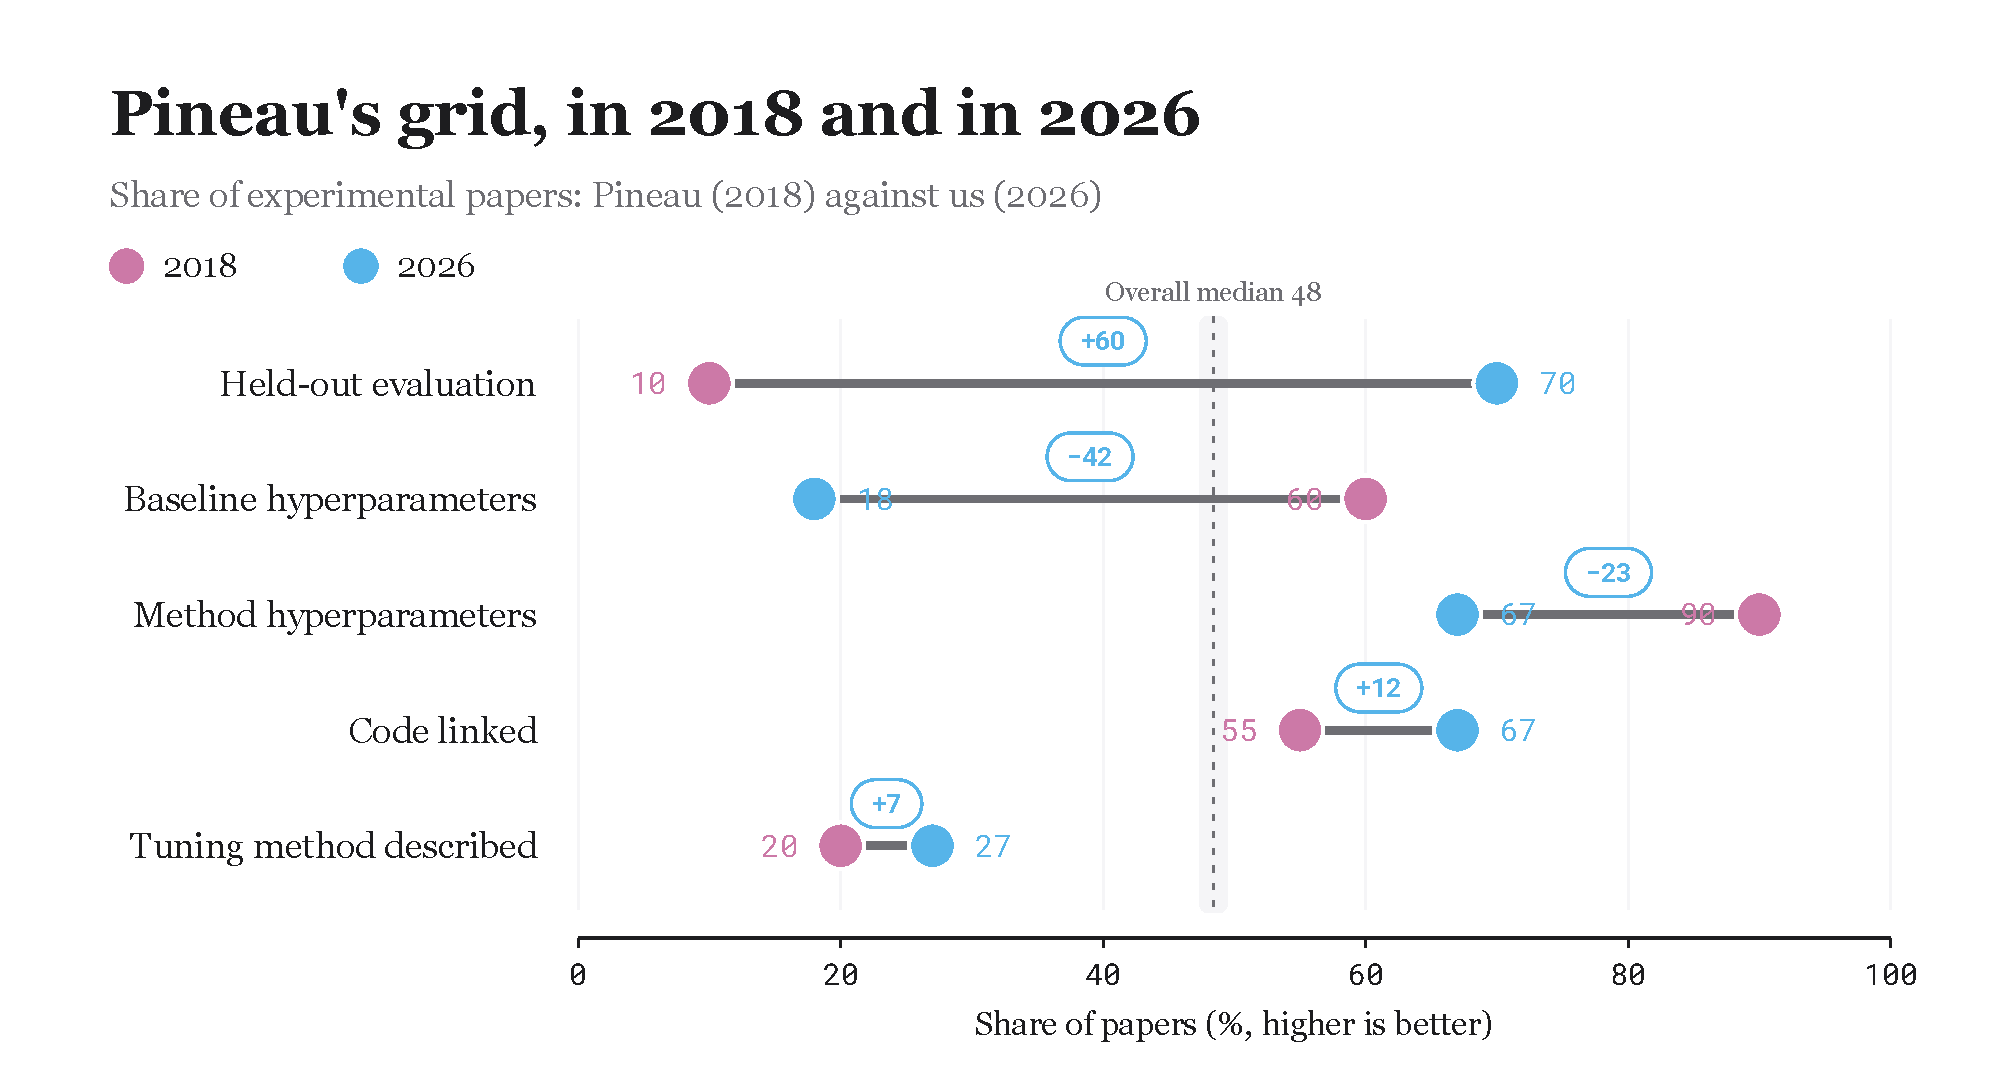
\includegraphics[width=1\linewidth,height=\textheight,keepaspectratio]{figures/remesure-dumbbell-en.pdf}
\caption{Joelle Pineau's grid for reading deep reinforcement learning
papers, applied in 2018 and in 2026. Each row is a reading criterion.
The 2018 dot gives the share of the 50 papers read by Pineau that meet
the criterion. The 2026 dot gives the share among our 45 experimental
papers drawn from three leading machine learning conferences (ICLR 2026,
ICML 2026 and NeurIPS 2025). The statistical test, left out of the
drawing, goes from 5\% to 4\%.}
\end{figure}

\begin{longtable}[]{@{}
  >{\raggedright\arraybackslash}p{(\linewidth - 8\tabcolsep) * \real{0.4868}}
  >{\raggedright\arraybackslash}p{(\linewidth - 8\tabcolsep) * \real{0.0658}}
  >{\raggedleft\arraybackslash}p{(\linewidth - 8\tabcolsep) * \real{0.1184}}
  >{\raggedleft\arraybackslash}p{(\linewidth - 8\tabcolsep) * \real{0.1447}}
  >{\raggedleft\arraybackslash}p{(\linewidth - 8\tabcolsep) * \real{0.1842}}@{}}
\caption{Joelle Pineau's grid for deep reinforcement learning papers,
reapplied criterion by criterion. The 2026 column gives a share with its
95\% Wilson confidence interval, in percent. In bold, the two changes
that hold against her figures and against our own reading of 2018. ``Not
measured'': Pineau did not have this criterion. Data:
\texttt{study/results\_final.json}.}\tabularnewline
\toprule\noalign{}
\begin{minipage}[b]{\linewidth}\raggedright
Reading criterion
\end{minipage} & \begin{minipage}[b]{\linewidth}\raggedright
Flaw targeted
\end{minipage} & \begin{minipage}[b]{\linewidth}\raggedleft
Pineau, 2018
\end{minipage} & \begin{minipage}[b]{\linewidth}\raggedleft
Our reading of 12 papers from 2018
\end{minipage} & \begin{minipage}[b]{\linewidth}\raggedleft
Our 45 papers from 2026, with 95\% interval
\end{minipage} \\
\midrule\noalign{}
\endfirsthead
\toprule\noalign{}
\begin{minipage}[b]{\linewidth}\raggedright
Reading criterion
\end{minipage} & \begin{minipage}[b]{\linewidth}\raggedright
Flaw targeted
\end{minipage} & \begin{minipage}[b]{\linewidth}\raggedleft
Pineau, 2018
\end{minipage} & \begin{minipage}[b]{\linewidth}\raggedleft
Our reading of 12 papers from 2018
\end{minipage} & \begin{minipage}[b]{\linewidth}\raggedleft
Our 45 papers from 2026, with 95\% interval
\end{minipage} \\
\midrule\noalign{}
\endhead
\bottomrule\noalign{}
\endlastfoot
Q5, the code is linked & F1 & 55\% & 6 of 11 & 67\% {[}52, 79{]} \\
Q3, all of the method's hyperparameters are given & F2, F4 & 90\% & 6 of
10 & 67\% {[}52, 79{]} \\
X7, the compute used is quantified & F2, F3 & not measured & 4 of 11 &
47\% {[}33, 61{]} \\
Q6, how the hyperparameters were chosen is described & F5 & 20\% & 2 of
10 & 27\% {[}16, 41{]} \\
Q4, all of the baselines' hyperparameters are given & F7 & 60\% & 6 of
11 & \textbf{18\% {[}10, 32{]}} \\
X4, the baselines are tuned with the same care & F7 & not measured & 4
of 10 & 5\% {[}1, 15{]} \\
X2, an uncertainty is reported & F12 & not measured & 8 of 11 & 47\%
{[}33, 61{]} \\
Q8, a statistical test is applied & F12 & 5\% & 1 of 11 & 4\% {[}1,
15{]} \\
Q7, evaluation uses held-out conditions & F15 & 10\% & 4 of 10 &
\textbf{70\% {[}56, 82{]}} \\
\end{longtable}

\textbf{Code, linked more often (F1).} In 2026, 67\% of papers link to
their code, against 55\% for Pineau. On our sample alone, the interval
{[}52, 79{]} settles nothing. The official report on the NeurIPS 2019
reproducibility programme points the same way: the share of accepted
papers with code rises from under 50\% to 74.4\%
\autocite{pineau2021improving}. So the flaw is partly heeded. One paper
in three remains an advertisement without the product.

\textbf{The plan for rerunning, half delivered (F2).} All of the
method's hyperparameters appear in 67\% of 2026 papers. The compute is
quantified in 47\%. The apparent drop for hyperparameters, from 90\% to
67\%, vanishes against our own reading of 2018 (6 of 10). Our grid is
simply stricter than Pineau's. The verdict remains impossible to settle.

\textbf{Infrastructure, quantified one time in two (F3).} Fewer than one
paper in two quantifies its compute in 2026, even though RL on large
models has turned compute into a budget line of its own
\autocite{khatri2025art}. Software versions (criterion Y10) await the
second grid.

\section{Tuning: hyperparameters and baselines (F4 to
F7)}\label{tuning-hyperparameters-and-baselines-f4-to-f7}

\textbf{How to tune, still left unsaid (F4 and F5).} How the
hyperparameters were chosen is described in 27\% of 2026 papers, against
20\% in 2018. The gap vanishes into the uncertainty: nothing has moved.

\textbf{Settings that change everything (F6).} The literature has
confirmed the observation of Henderson and co-authors at large scale. In
2020, a team at MIT (Massachusetts Institute of Technology) shows that
code details absent from the papers explain a good part of the advantage
credited to PPO \autocite{engstrom2020implementation}. In 2021, a Google
team trains 250,000 agents to measure the effect of each choice
\autocite{andrychowicz2021matters}. Whether 2026 papers show their own
sensitivity to settings is still open: criterion Y9 will tell.

\textbf{Baselines, described less and less (F7).} On this flaw, practice
has clearly slipped back. All of the baselines' hyperparameters are
given in 18\% of 2026 papers, against 60\% for Pineau and 6 of 11 in our
reading of 2018. Only 5\% of papers say they tuned their baselines with
the same care as their method. Our sample says nothing about the cause
of this decline.

\textbf{The badly tuned baseline was us.} Our experiment E6 set out to
illustrate the flaw. It pits PPO on Hopper with the library's default
values against PPO with the settings published by the RL Baselines3 Zoo
collection \autocite{raffin2020zoo}, the reference settings for this
library. On the first pass, the default version reaches an interquartile
mean of 2,877 (interval 2,272 to 3,346), the tuned version 1,003
(interval 859 to 1,156). The interquartile mean (IQM) discards the
lowest quarter and the highest quarter of the runs, then averages the
rest \autocite{agarwal2021precipice}. Did the published settings really
do three times worse than the defaults? The result made our point too
neatly, in reverse. We checked. Our code normalised observations with a
discount factor of 0.99, while the collection uses the algorithm's own
factor, 0.999. The badly tuned baseline was us. The first pass is kept
as it is in the results. We reran the corrected recipe with ten random
seeds per condition, on Hopper in its versions 4 and 5. We decided on
this diagnosis after seeing the first result, as the protocol declares.
All thirty runs are finished. The analysis is still to do.

\section{Random seeds and statistics (F8 to
F12)}\label{random-seeds-and-statistics-f8-to-f12}

\textbf{The measure, still to be defined (F8).} Criterion Y1 will tell
whether 2026 papers define their performance measure, criterion Y2
whether they state what their error bars represent.

\textbf{Still five runs (F9).} Of 41 experimental RL papers from 2026,
20 leave unstated how many independent training runs support their
results. Four have only one. The median among the others is five, the
figure Pineau noted in 2018. The flaw was not heeded. Experiment E5 will
tell how many random seeds it really takes.

\subsection{Same code, another random seed
(F11)}\label{same-code-another-random-seed-f11}

We redid the most famous experiment of 2018 at a larger scale: thirty
training runs of PPO on HalfCheetah, a million steps each, with the same
code and the same hyperparameters. Only the random seed changes.

\begin{figure}
\centering
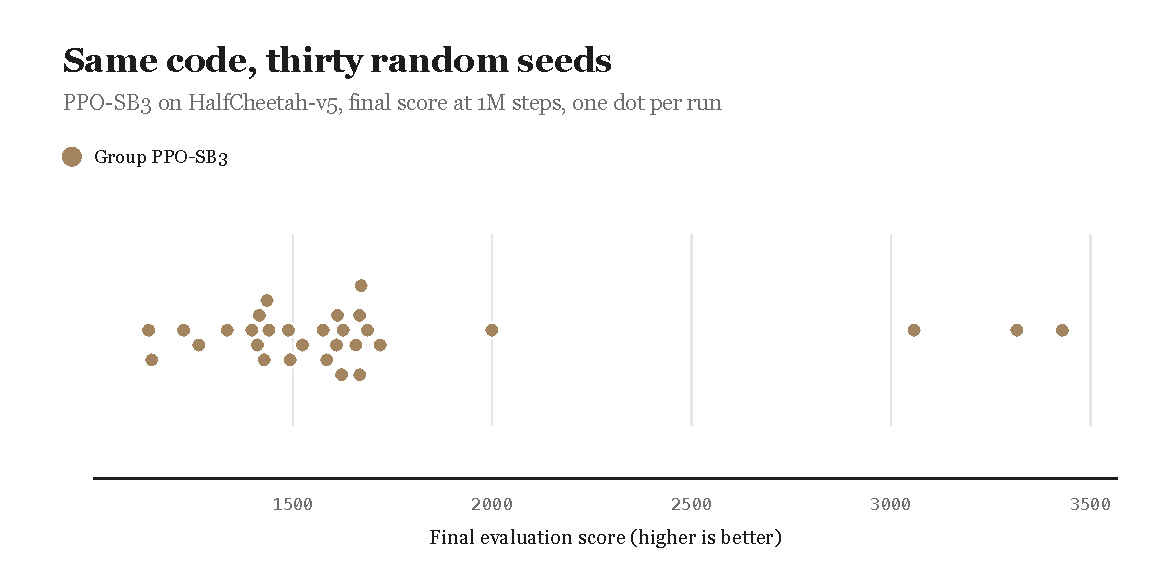
\includegraphics[width=1\linewidth,height=\textheight,keepaspectratio]{figures/e1-seeds-en.pdf}
\caption{Thirty training runs of the same program on the same task (the
PPO algorithm, Proximal Policy Optimization, on the HalfCheetah
simulated cheetah). Each dot is a run, placed at the height of its final
evaluation score. Only the random seed changes from one dot to the next.
Mean 1,688, standard deviation 568, median 1,580. Twenty-seven runs end
between 1,138 and 1,999. Three take off beyond 3,000.}
\end{figure}

\textbf{A spread that looks nothing like a bell.} The standard deviation
equals 34\% of the mean. The distribution strays far from the bell
curve: a Shapiro-Wilk test, which measures this departure, gives p = 4 ×
10\textsuperscript{−7}. Three runs out of thirty take off far above the
others.

\textbf{How often does chance fool the test?} We then drew two groups
from the thirty runs 10,000 times and applied Welch's test, the classic
test for comparing two means, to each pair
\autocite{welch1947generalization}. Since both groups come from the same
program, every gap declared significant is a false positive.

\begin{figure}
\centering
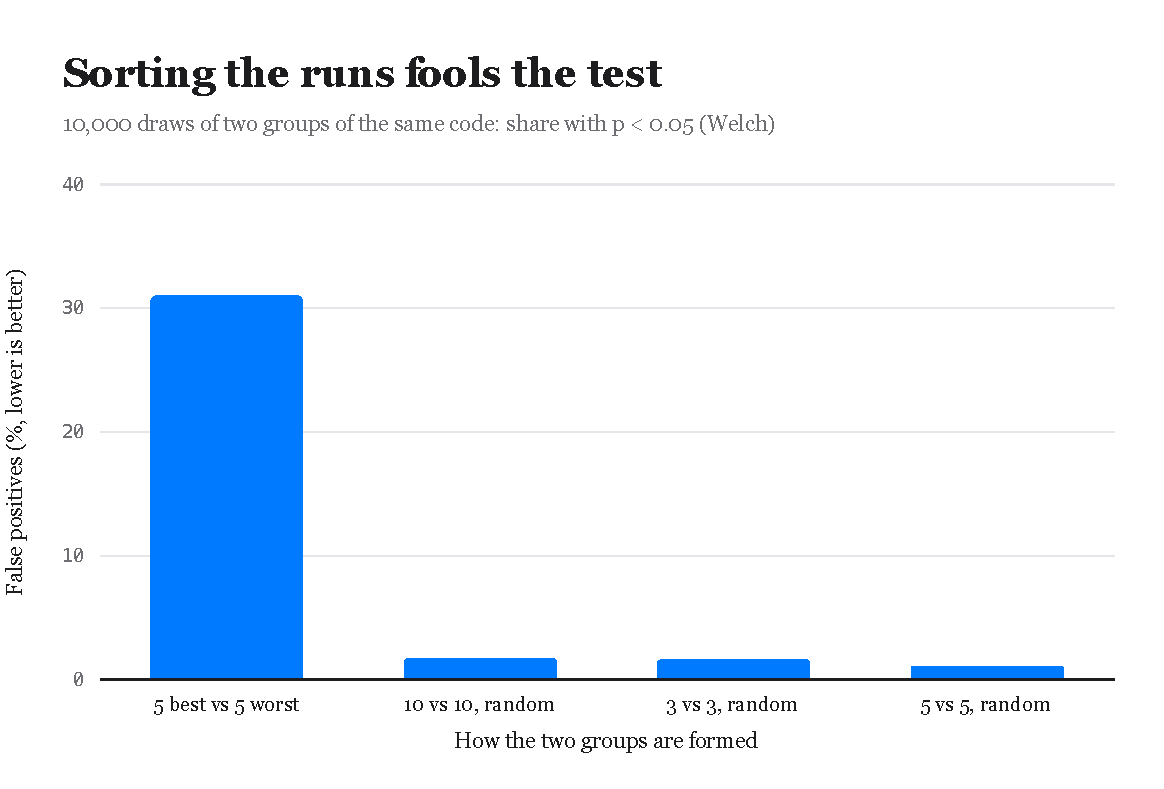
\includegraphics[width=0.9\linewidth,height=\textheight,keepaspectratio]{figures/e1-false-positive-en.pdf}
\caption{Share of 10,000 draws in which Welch's test declares two groups
of runs from the same program different, at the 5\% threshold. When the
groups are drawn at random, the test errs less often than that
threshold. When ten runs are sorted and the five best are set against
the five worst, the test errs nearly one time in three.}
\end{figure}

\begin{longtable}[]{@{}
  >{\raggedright\arraybackslash}p{(\linewidth - 6\tabcolsep) * \real{0.5217}}
  >{\raggedleft\arraybackslash}p{(\linewidth - 6\tabcolsep) * \real{0.1594}}
  >{\raggedleft\arraybackslash}p{(\linewidth - 6\tabcolsep) * \real{0.1594}}
  >{\raggedleft\arraybackslash}p{(\linewidth - 6\tabcolsep) * \real{0.1594}}@{}}
\caption{Experiment E1, 10,000 draws per row, all from thirty runs of
one program (PPO on HalfCheetah) that differ only by their random seed.
The apparent gap divides the difference between the two means by the
smaller of the two. Data: \texttt{sim/analysis/e1.json}.}\tabularnewline
\toprule\noalign{}
\begin{minipage}[b]{\linewidth}\raggedright
How the two groups are formed
\end{minipage} & \begin{minipage}[b]{\linewidth}\raggedleft
Share of draws declared different (p \textless{} 0.05)
\end{minipage} & \begin{minipage}[b]{\linewidth}\raggedleft
Apparent gap between the means, median
\end{minipage} & \begin{minipage}[b]{\linewidth}\raggedleft
Apparent gap exceeded one time in twenty
\end{minipage} \\
\midrule\noalign{}
\endfirsthead
\toprule\noalign{}
\begin{minipage}[b]{\linewidth}\raggedright
How the two groups are formed
\end{minipage} & \begin{minipage}[b]{\linewidth}\raggedleft
Share of draws declared different (p \textless{} 0.05)
\end{minipage} & \begin{minipage}[b]{\linewidth}\raggedleft
Apparent gap between the means, median
\end{minipage} & \begin{minipage}[b]{\linewidth}\raggedleft
Apparent gap exceeded one time in twenty
\end{minipage} \\
\midrule\noalign{}
\endhead
\bottomrule\noalign{}
\endlastfoot
3 runs against 3, drawn at random & 1.6\% & 17\% & 62\% \\
5 runs against 5, drawn at random & 1.2\% & 17\% & 47\% \\
10 runs against 10, drawn at random & 1.7\% & 11\% & 33\% \\
The 5 best against the 5 worst, out of 10 runs & 31.0\% & 42\% & not
computed \\
\end{longtable}

\textbf{Chance fools the eye, sorting fools the test.} Two groups of
five runs drawn at random almost never fool the test (1.2\%). They do
fool the eye: their means differ by 17\% at the median and by 47\% one
time in twenty, enough to draw two well-separated curves. The test goes
wrong when the runs are sorted: setting the five best runs against the
five worst gives 31\% false positives. The 2018 figure probably belongs
to this second case. The caption by Henderson and co-authors specifies
that their p is an average of tests run along the learning curve. Their
paper does not say how the ten runs were split into two groups
\autocite{henderson2018matters}. So our measurement qualifies the flaw.
The flaw still stands: a reader who looks at two curves without an
interval falls into the trap of the eye.

\textbf{Best of N, now rare (F10).} In E1, keeping the three best runs
out of ten inflates the mean by 33\% (2,249 against 1,692). In 2026
papers, the practice has become rare or hidden: 2 papers out of 45 let
it show. Experiment E4 will tell how many comparisons between algorithms
it reverses.

\textbf{Statistics, still missing (F12).} The statistical test remains
at 4\% of papers, against 5\% in 2018. An uncertainty is reported in
47\% of papers, though this average mixes two worlds. Classical RL
always reports it (14 papers out of 14). RL on large models almost never
does (4 out of 27), even though a team from Tübingen and Cambridge
measured there, in 2025, standard deviations of 5 to 15 percentage
points from one random seed to the next \autocite{hochlehnert2025sober}.

\begin{figure}
\centering
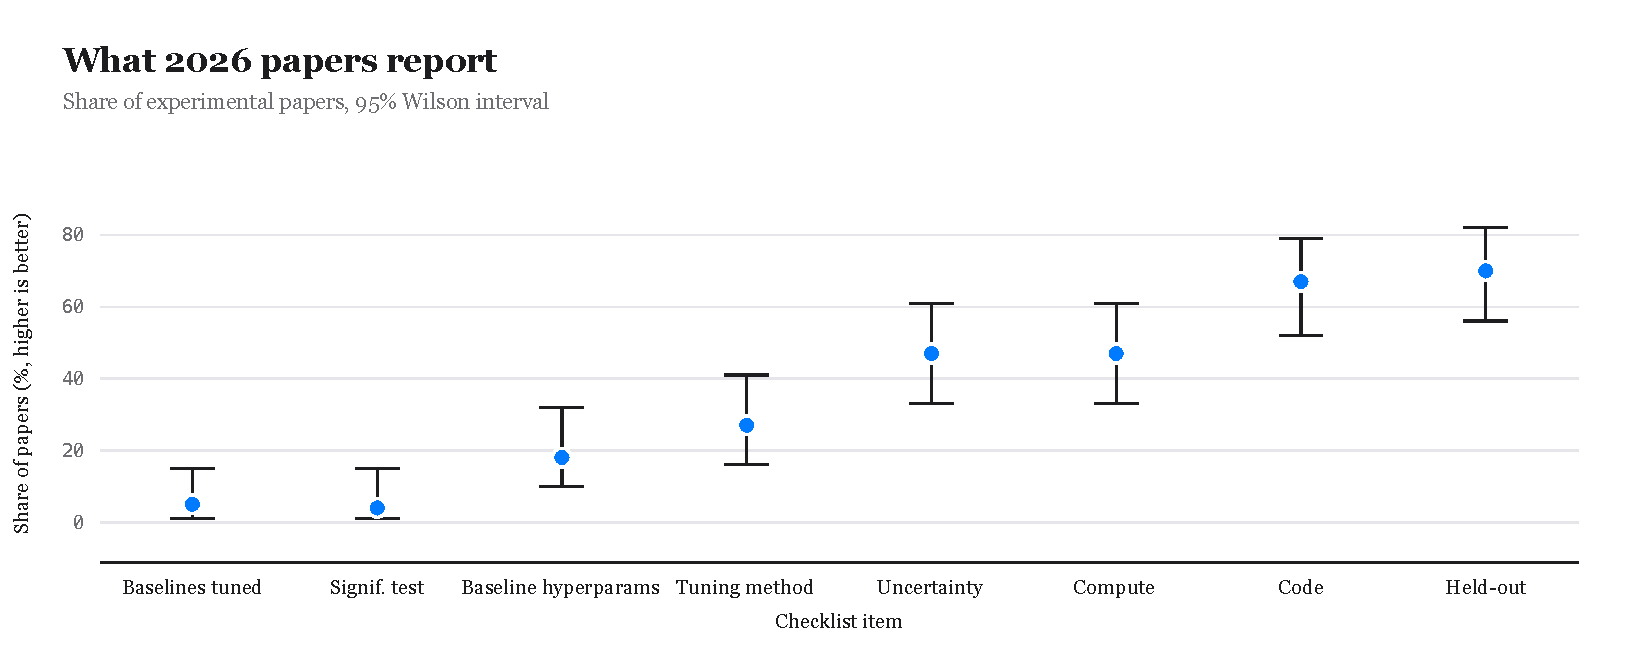
\includegraphics[width=1\linewidth,height=\textheight,keepaspectratio]{figures/remesure-ic-en.pdf}
\caption{Share of the 2026 deep reinforcement learning papers that meet
each reading criterion, with its 95\% Wilson confidence interval. The
vertical bars show the range compatible with our 45 experimental papers.
With a sample this size, a gap of under fifteen points from 2018 blends
into the luck of the draw.}
\end{figure}

\section{The reach of the conclusions (F13 to
F16)}\label{the-reach-of-the-conclusions-f13-to-f16}

\textbf{Rankings and implementations (F13 and F14).} Experiment E2 ranks
four algorithms on four tasks. E3 compares PPO written in PyTorch with
PPO written in JAX, using the same random seeds. Both await the end of
the simulations. Criteria Y3 to Y5 will tell whether 2026 papers test
several tasks, show those where their method loses and say where the
code of their baselines comes from.

\textbf{Held-out evaluation, the best-heeded flaw (F15).} In 2026, 70\%
of papers evaluate on held-out conditions, against 10\% in 2018. The
progress comes mostly from RL on large models: 26 papers out of 27.
Their benchmarks, collections of mathematics problems, separate training
problems from test problems by construction. Classical RL stays at 5
papers out of 13. Experiment E7 measures, on our own agents, what
modified physics costs.

\textbf{Benchmarks too simple, in another form (F16).} RL on large
models has changed scale without changing risk. Fifteen papers out of 27
try a single family of language models. Yet a University of Washington
team showed in 2025 that a reward drawn at random improves Qwen models
in mathematics, but not Llama or OLMo models
\autocite{shao2025spurious}. A result obtained on a single family
informs about that family and proves nothing about the method.

\textbf{A length limit that distorts the gain.} Our GRPO strand brought
a benchmark trap to light. The model's answers are cut off at 160
tokens, the word pieces the model produces one by one. With the starting
model, 23 answers out of 32 hit this limit before giving a result. Every
one of these cut-off answers is wrong. With the true reward, the model
first learns to finish before the cut, a lesson the random reward never
teaches. Part of the measured ``gain'' therefore comes from a detail of
the benchmark. We now measure the share of cut-off answers at every
evaluation.

\begin{figure}
\centering
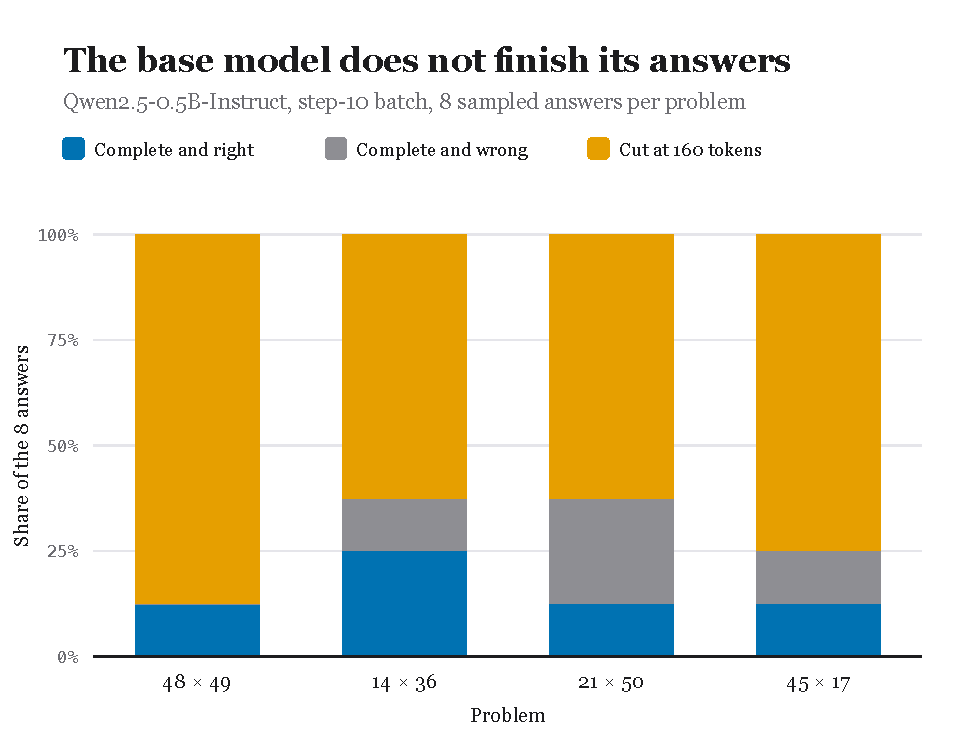
\includegraphics[width=0.8\linewidth,height=\textheight,keepaspectratio]{figures/grpo-truncation-en.pdf}
\caption{Answers of the Qwen2.5 language model with 0.5 billion
parameters, before any training, on the four multiplication problems of
the tenth step of our pilot run. The model drew eight answers per
problem. Most hit the 160-token length limit before giving a result and
are scored as wrong.}
\end{figure}

\textbf{Three GRPO runs finished.} Of the twelve planned runs, three
completed, all on Qwen. With the true reward, first-attempt success
rises from 10\% and 12\% to 36\% and 61\% in a hundred steps. With the
random reward, success falls to 1\%. The other nine runs failed when
they were restarted on 9 November 2026, for computing reasons recorded
in the protocol. A single random seed per condition supports no
conclusion.

\section{The remedies: a checklist and a reproducibility
challenge}\label{the-remedies-a-checklist-and-a-reproducibility-challenge}

\textbf{The checklist.} Pineau went beyond the diagnosis. She proposed a
reproducibility checklist (pages 31 to 33 at NeurIPS). For each
algorithm, it asks for a clear description, a complexity analysis, the
link to the code and its dependencies. For each theoretical result, it
asks for the statement, the assumptions and the proof. For each figure,
it asks for how the data were collected, the split between training,
validation and test, the excluded data, the range and method used to
choose the hyperparameters, the exact number of runs, the definition of
the statistics and error bars, the hardware used.

\textbf{The reproducibility challenge.} She also presented the ICLR 2018
reproducibility challenge (slides 37 to 43 at ICLR): students around the
world tried to redo submitted papers. Participants chose 95 papers. Of
the participants, 54.5\% reproduced part of a paper and 32.7\%
reproduced most of it. Among the authors, 61\% said they were willing to
correct their paper.

\textbf{What the checklist changed.} The checklist won over the
institution: NeurIPS has required it since 2019
\autocite{pineau2021improving}. Our grid says what it changed in the
papers. Code sharing improved a little and held-out evaluation a lot.
Statistics stayed where they were. The description of baselines moved
the wrong way. A checklist gets boxes ticked. Launching ten random seeds
and tuning one's baselines costs compute. The checklist pays for none of
it.

\section{Related work}\label{related-work}

\textbf{A measurement nobody has repeated.} We searched arXiv,
OpenReview and the conference proceedings on 9 November 2026. To our
knowledge, no work reapplies Pineau's grid to recent RL papers while
calibrating it on 2018. None reruns the protocol of Henderson and
co-authors with 2026 algorithms under a protocol written in advance.
Neighbouring pieces exist: they situate our contribution.

\textbf{Audits of the literature.} In 2018, Gundersen and Kjensmo scored
400 papers from the IJCAI (International Joint Conference on Artificial
Intelligence) and AAAI (Association for the Advancement of Artificial
Intelligence) conferences on how they document methods, data and
experiments \autocite{gundersen2018state}. In 2026, Coakley and
co-authors tracked 56,800 papers from five artificial intelligence
conferences from 2014 to 2024: the share that releases code and data
rises from 11\% to 64\%. The rise begins before the checklists
\autocite{coakley2026shift}. Magnusson and co-authors measure the effect
of the checklist adopted by natural language processing conferences
\autocite{magnusson2023nlpchecklist}. In RL, the closest audit is the
one by Gorsane and co-authors: 75 papers on cooperative multi-agent RL
from 2016 to 2022, about a third of which quantify no uncertainty
\autocite{gorsane2022marl}. All these audits leave aside single-agent RL
and the 2018 grid.

\textbf{Statistical method.} Colas and co-authors compute how many
random seeds it takes to detect a given gap \autocite{colas2018seeds}.
Jordan and co-authors discuss the measure itself
\autocite{jordan2020evaluating,jordan2024position}. Agarwal and
co-authors contribute the interquartile mean and intervals computed by
resampling \autocite{agarwal2021precipice}. Patterson and co-authors
turn this into a guide \autocite{patterson2024empirical}. Eimer and
co-authors call for the same tuning budget for baselines as for the
method \autocite{eimer2023hyperparameters}. These works say what to do.
Our survey measures whether the community does it.

\textbf{Experiments redone.} Islam and co-authors preceded Henderson on
the same tasks \autocite{islam2017reproducibility}. Lynnerup and
co-authors rerun algorithms on a real robot arm
\autocite{lynnerup2020survey}. Bjorck and co-authors show that part of
the variance between random seeds comes from training runs that fail
completely. They then reduce that variance
\autocite{bjorck2022variance}. Our three outlying runs in E1 belong to
this phenomenon in reverse: three training runs that succeed far better
than the rest.

\textbf{RL on large models.} Hochlehnert and co-authors re-evaluate
reasoning models and find large gaps from one random seed to the next
\autocite{hochlehnert2025sober}. Chandak and co-authors report, in a
blog post that was not peer-reviewed, starting models under-evaluated in
seven papers \autocite{chandak2025incorrect}: the modern equivalent of
the badly tuned baselines of 2018. Shao and co-authors show the random
reward that ``works'' \autocite{shao2025spurious}. Our GRPO strand
illustrates this last result without claiming to discover it.

\textbf{Our contribution.} It comes from combining three pieces. A
before-and-after measurement uses the original grid, calibrated by our
own reading of 2018. The experiments of 2018 are redone with the tools
of 2026 under a protocol written in advance. A bridge finally links this
work to RL on large models.

\section{What we take from it}\label{what-we-take-from-it}

\textbf{Partly heeded, in an unexpected place.} The best-corrected flaw,
held-out evaluation, was corrected mostly because RL changed terrain:
collections of mathematics problems come with a test set by
construction. The flaws that demanded effort with no outside constraint
stagnated or slipped back: ten random seeds, a statistical test,
baselines tuned like the method.

\textbf{Chance fools the eye, our choices fool the test.} Our
experiments qualify the most famous figure of 2018. Random seeds
manufacture visible gaps. Our choices, sorting the runs and keeping the
best, turn those gaps into false positives. We draw two rules from this.
Never sort the random seeds. Show an interval next to every curve.

\textbf{The grid applies to oneself first.} We badly tuned the baseline
we meant to show as badly tuned. Our first GRPO indicator was measuring
a length limit. We found both errors because the protocol was written in
advance and because we checked surprising results before publishing
them. That was Pineau's advice in 2018: be as critical of your good
results as of your bad ones.

\section{Limitations}\label{limitations}

\textbf{The size of the survey.} With 50 papers, the intervals stay
wide: only a gap of more than fifteen points from 2018 reads without
ambiguity. Our reading of 2018 is stricter than Pineau's on the method's
hyperparameters.

\textbf{Flaws still unmeasured.} Six flaws (F6, F8, F13, F14, F16 and
part of F3) await the second grid or the end of the simulations. E1 is
limited to one task and one algorithm. The GRPO strand remains an
illustration on models of 0.5 and 1 billion parameters, far from a
replication of Shao and co-authors.

\section{What remains to be measured}\label{what-remains-to-be-measured}

\begin{itemize}
\tightlist
\item
  The second grid (Y1 to Y12) goes to the 50 papers from 2026 and the 12
  from 2018, with the same rules and a double reading of 10 papers. Its
  plan is written.
\item
  Experiments E2 to E5 and E7 follow once the 75 remaining training runs
  finish. The analysis of E6 comes next, since its runs are complete.
\item
  The nine remaining GRPO runs restart overnight, with the share of
  cut-off answers measured at every evaluation.
\end{itemize}

\section{Reproducibility}\label{reproducibility}

The code, the protocols, the evaluation logs and the analysis scripts
are in \texttt{study/}, \texttt{sim/} and \texttt{sim/llm/}. The script
\texttt{docs/figures/build.py} regenerates every figure from the results
files. The software environment is frozen in
\texttt{sim/requirements.lock}.

\printbibliography[title={References}]
\end{document}
